% !TeX root = ../main.tex
\documentclass[./../main.tex]{subfiles}

\begin{document}
Ở chương trước, tôi đã giới thiệu về quy trình phát hiện một tài liệu PDF độc hại, gồm hai phần chính là trích xuất đặc trưng và phân loại dữ liệu. Chương hai này sẽ tiến hành thử nghiệm, từ cài đặt công cụ trích xuất đặc trưng trên tập dữ liệu thu thập được đến xây dựng mô hình học máy mang lại độ chính xác cao khi phân loại một tệp sạch hay độc hại.

\section{Tập dữ liệu}
Tập dữ liệu bao gồm 22046 tệp PDF riêng biệt, với tỉ lệ tệp độc là 58\%, tệp sạch là 42\%, không gây sự chênh lệch quá lớn trên hai nhãn. Trong đó số lượng tài liệu có nhúng javascript chiếm 75\%. Toàn bộ tập dữ liệu là kết quả của quá trình thu thập và loại bỏ tệp trùng lặp từ một số nguồn như Contagio, Evasive-PDFMal2022 và VirusTotal. Với VirusTotal, thực hiện truy vấn để tìm kiếm các tệp PDF độc hại có nhúng javascript và được gán nhãn CVE có độ nguy hiểm cao. Một số CVE được thu thập trong các tài liệu PDF độc như CVE-2007-5659, CVE-2008-2992, CVE-2009-4324, CVE-2010-0188,...

\begin{table}[]
	\centering
	\caption{Thống kê số lượng tệp dữ liệu có chứa javascript.}
	\label{tab:data_contain_javascript}
	\begin{tabular}{|l|c|c|c|}
		\hline
		        & contain js & no contain js & total \\ \hline
		malware & 12183      & 584           & 12767 \\ \hline
		benign  & 4326       & 4953          & 9279  \\ \hline
	\end{tabular}
\end{table}

Các tệp PDF sau khi được xử lý qua quá trình trích xuất đặc trưng, sẽ được phân chia thành các tập dữ liệu phục vụ quá trình huấn luyện và kiểm định. Với mô hình yêu cầu một tập validation phục vụ cho quá trình điều chỉnh tham số hay lựa chọn bộ đặc trưng tốt, sự phân chia sẽ theo tỉ lệ 7:2:1 với 70\% là tập huấn luyện, 20\% là tập kiểm chứng, 10\% là tập kiểm thử.

\begin{table}[]
	\centering
	\caption{Phân bổ tập huấn luyện, kiểm chứng và tập kiểm thử}
	\label{tab:phan_bo_tap_huan_luyen}
	\begin{tabular}{|l|c|}
		\hline
		               & Samples \\ \hline
		Training set   & 15431   \\ \hline
		Validation set & 4409    \\ \hline
		Test set       & 2205    \\ \hline
	\end{tabular}
\end{table}

\section{Trích xuất đặc trưng}
\subsection{Đặc trưng thống kê}
Các đặc trưng thống kê là các đặc trưng được trích xuất từ quá trình phân tích cú pháp, cấu trúc của tệp PDF, mang ý nghĩa thống kê như đếm số lượng từ khóa xuất hiện trong tài liệu, phân tích tương quan giữa các giá trị, số lượng bộ lọc được sử dụng...

Trình đọc PDF sử dụng các từ khóa được nhúng trong tài liệu, theo sau bởi ký tự ‘\slash’ để hiểu những hành động cần thực thi, do đó tập hợp những từ khóa có thể là các chỉ báo hiệu quả về hành vi của tài liệu. Một số từ khóa có thể có liên quan chặt chẽ tới một số lỗ hổng hoặc hành vi độc hại, điển hình như ‘\slash JS’ hay ‘\slash Javascript’ chỉ ra có đoạn mã javascript được nhúng trong tài liệu, những đoạn mã này có độ nguy hiểm cao bởi xuất hiện trong hầu hết các cuộc tấn công mã độc; hay ‘\slash URI’: cho phép truy cập một nguồn từ xa, bằng cách này, kẻ tấn công có thể chuyển hướng người dùng tới một trang web độc hại.

Tài liệu PDF hỗ trợ một số các bộ lọc phục vụ nén, mã hóa dữ liệu. Những kẻ tấn công có thể lợi dụng bộ lọc để ẩn các đoạn mã độc hại và che giấu hành vi. Do đó, việc xác định những bộ lọc nào được sử dụng, những bộ lọc nào thường xuất hiện trong tệp độc hại hay tệp sạch sẽ mang lại những đặc trưng có giá trị trong việc phân loại tệp.

Ngoài ra đặc trưng thống kê cũng bao gồm các metafeatures - các đặc trưng phản ánh phần nào các thuộc tính của siêu dữ liệu, ví dụ như số lượng các từ viết hoa trong trường tác giả, hay tỉ lệ của số trang trên kích thước tài liệu.

Thông qua việc kết hợp sử dụng hai công cụ PeePDF và PDFiD, dưới đây là tập các đặc trưng thống kê được lựa chọn trích xuất [ref bảng]. Bộ đặc trưng này gồm có 67 đặc trưng.

% Please add the following required packages to your document preamble:
% \usepackage{longtable}
% Note: It may be necessary to compile the document several times to get a multi-page table to line up properly
\begin{longtable}[c]{|p{.4\textwidth}|p{.6\textwidth}|}
	\caption{Danh sách 67 đặc trưng thống kê và mô tả}
	\label{tab:danh_sach_bang_67_dac_trung}                                                                                                                                 \\
	\hline
	\textbf{Tên đặc trưng}                    & \textbf{Mô tả}                                                                                                              \\ \hline
	\endfirsthead
	%
	\endhead
	%
	file\_size                                & Kích thước tệp                                                                                                              \\ \hline
	pdfid\_check\_isPDF                       & Kiểm tra xem tệp có phải là tài liệu PDF hay không                                                                          \\ \hline
	is\_linearized                            & Đặc trưng này dùng để kiểm tra tệp có là Linearized PDF hay không                                                           \\ \hline
	is\_encrypted                             & Kiểm tra xem tệp có bị mã hóa hay không                                                                                     \\ \hline
	pdf\_version                              & Phiên bản tài liệu PDF                                                                                                      \\ \hline
	num\_updates                              & Số lần tệp PDF được cập nhật                                                                                                \\ \hline
	num\_objects                              & Số lượng đối tượng xuất hiện trong tệp                                                                                      \\ \hline
	num\_streams                              & Số lượng các đối tượng stream                                                                                               \\ \hline
	peepdf\_num\_errors                       & Số lượng lỗi khi phân tích cú pháp tệp qua công cụ PeePDF                                                                   \\ \hline
	pdfid\_error\_occured                     & Kiểm tra tệp có bị lỗi khi phân tích qua công cụ PDFiD hay không                                                            \\ \hline
	bad\_pdf\_header                          & Kiểm tra sự không hợp lệ của header tệp PDF                                                                                 \\ \hline
	num\_comments                             & Số lượng comment trong tệp                                                                                                  \\ \hline
	num\_indirect\_objects                    & Số lượng đối tượng tham chiếu trong tệp                                                                                     \\ \hline
	num\_compressed\_objects                  & Số lượng các đối tượng được nén                                                                                             \\ \hline
	num\_encode\_streams                      & Số lượng stream được mã hóa                                                                                                 \\ \hline
	num\_decode\_streams\_error               & Số lượng lỗi xuất hiện khi thực hiện giải mã những stream bị mã hóa                                                         \\ \hline
	num\_error\_objects                       & Số lượng các đối tượng lỗi                                                                                                  \\ \hline
	num\_object\_streams                      & Số lượng các stream chứa đối tượng                                                                                          \\ \hline
	num\_xref\_streams                        & Số lượng xref stream (từ phiên bản 1.5, tệp PDF cho phép bảng tham chiếu được lưu dưới dạng stream với từ khóa /ObjStm)     \\ \hline
	num\_objects\_contain\_js                 & Số lượng đối tượng chứa đoạn mã javascript                                                                                  \\ \hline
	num\_\%\%EOF                              & Số lần xuất hiện của từ khóa đánh dấu sự kết thúc của tệp PDF                                                               \\ \hline
	char\_after\_last\_EOF                    & Số lượng ký tự sau từ khóa kết thúc cuối cùng trong tệp PDF                                                                 \\ \hline
	stream\_entropy\_less\_than\_2            & Kiểm tra xem entropy của tệp có nhỏ hơn 2 hay không (entropy tính toán sự phân bổ ngẫu nhiên của các bytes trong chuỗi)     \\ \hline
	total\_file\_entropy                      & Giá trị entropy của toàn bộ tệp                                                                                             \\ \hline
	stream\_entropy                           & Giá trị entropy bên trong các đối tượng stream                                                                              \\ \hline
	non\_stream\_entropy                      & Giá trị entropy của các chuỗi bên ngoài stream                                                                              \\ \hline
	obj                                       & Số lần xuất hiện của từ khóa 'obj', từ khóa xác định sự bắt đầu của một đối tượng                                           \\ \hline
	endobj                                    & Số lần xuất hiện của từ khóa 'endobj', từ khóa xác định sự kết thúc của một đối tượng                                       \\ \hline
	stream                                    & Số lần xuất hiện của từ khóa 'stream', từ khóa xác định sự bắt đầu của một stream                                           \\ \hline
	endstream                                 & Số lần xuất hiện của từ khóa 'endstream', từ khóa xác định sự kết thúc của một stream                                       \\ \hline
	xref                                      & Số lần xuất hiện của từ khóa 'xref', từ khóa xác định sự bắt đầu của bảng tham chiếu tới vị trí các đối tượng trong tệp PDF \\ \hline
	trailer                                   & Số lần xuất hiện của từ khóa 'trailer', từ khóa xác định trailer của tệp PDF                                                \\ \hline
	startxref                                 & Số lần xuất hiện của từ khóa 'startxref', từ khóa xác định vị trí bắt đầu của bảng tham chiếu.                              \\ \hline
	/Page                                     & Số lần xuất hiện của từ khóa 'Page', xác định một trang của tệp PDF                                                         \\ \hline
	/Encrypt                                  & Số lần xuất hiện của từ khóa 'Encrypt'                                                                                      \\ \hline
	/ObjStm                                   & Số lần xuất hiện của từ khóa 'ObjStm'                                                                                       \\ \hline
	/JS                                       & Số lần xuất hiện của từ khóa 'JS', xác định đoạn mã javascript                                                              \\ \hline
	/JavaScript                               & Số lần xuất hiện của từ khóa 'JavaScript', tương tự như từ khóa 'JS                                                         \\ \hline
	/AA                                       & Số lần xuất hiện của từ khóa 'AA', xác định các hành động bổ sung, các sự kiện kích hoạt một hành vi nào đó                 \\ \hline
	/OpenAction                               & Số lần xuất hiện của từ khóa 'OpenAction', xác định hành động sẽ được thực thi ngay sau khi tệp PDF được mở                 \\ \hline
	/AcroForm                                 & Số lần xuất hiện của từ khóa 'AcroForm', xác định các phần tử biểu mẫu tương tác                                            \\ \hline
	/Names                                    & Số lần xuất hiện của từ khóa 'Names'                                                                                        \\ \hline
	/RichMedia                                & Số lần xuất hiện của từ khóa 'RichMedia', thường chứa embedded flash                                                        \\ \hline
	/Launch                                   & Số lần xuất hiện của từ khóa 'Launch', được sử dụng để mở một thực thể bên ngoài, có thể là một tệp thực thi.               \\ \hline
	/XFA                                      & Số lần xuất hiện của từ khóa 'XFA'                                                                                          \\ \hline
	/JBIG2Decode                              & Số lần xuất hiện của từ khóa 'JBIG2Decode'                                                                                  \\ \hline
	/U3D                                      & Số lần xuất hiện của từ khóa 'U3D'                                                                                          \\ \hline
	/PRC                                      & Số lần xuất hiện của từ khóa 'PRC'                                                                                          \\ \hline
	/Flash                                    & Số lần xuất hiện của từ khóa 'Flash'                                                                                        \\ \hline
	/SubmitForm                               & Số lần xuất hiện của từ khóa 'SubmitForm'                                                                                   \\ \hline
	/ImportData                               & Số lần xuất hiện của từ khóa 'ImportData'                                                                                   \\ \hline
	Colors \textgreater 2\textasciicircum{}24 & Số lượng màu có kích thước lớn hơn 2\textasciicircum{}24 (hơn 3 bytes)                                                      \\ \hline
	combination\_js\_and\_action              & Kiểm tra sự xuất hiện đồng thời của các đoạn mã javascript và các hành động khởi chạy                                       \\ \hline
	num\_EmbeddedFile                         & Số lượng tệp được nhúng trong tài liệu PDF                                                                                  \\ \hline
	num\_URI                                  & Số lần xuất hiện của từ khóa 'URI', đường dẫn tới một nguồn từ xa, có thể là một trang web                                  \\ \hline
	num\_ASCIIHexDecode                       & Số lần sử dụng thuật toán giải mã ASCIIHexDecode                                                                            \\ \hline
	num\_ASCII85Decode                        & Số lần sử dụng thuật toán giải mã ASCII85Decode                                                                             \\ \hline
	num\_LZWDecode                            & Số lần sử dụng thuật toán giải mã LZWDecode                                                                                 \\ \hline
	num\_FlateDecode                          & Số lần sử dụng thuật toán giải mã FlateDecode                                                                               \\ \hline
	num\_RunLengthDecode                      & Số lần sử dụng thuật toán giải mã RunLengthDecode                                                                           \\ \hline
	num\_CCITTFaxDecode                       & Số lần sử dụng thuật toán giải mã CCITTFaxDecode                                                                            \\ \hline
	num\_JBIG2Decode                          & Số lần sử dụng thuật toán giải mã JBIG2Decode                                                                               \\ \hline
	num\_DCTDecode                            & Số lần sử dụng thuật toán giải mã DCTDecode                                                                                 \\ \hline
	num\_JPXDecode                            & Số lần sử dụng thuật toán giải mã JPXDecode                                                                                 \\ \hline
	num\_Crypt                                & Số lượng stream bị mã hóa                                                                                                   \\ \hline
	num\_stream\_filters                      & Số lượng bộ lọc được sử dụng                                                                                                \\ \hline
	num\_unknown\_stream\_filters             & Số lượng bộ lọc được sử dụng nhưng không trong danh sách các bộ lọc được hỗ trợ của tài liệu PDF                            \\ \hline
\end{longtable}
\subsection{Đặc trưng cấu trúc cây}
Như đề cập ở mục 1.1.3, các đối tượng của tệp PDF được tổ chức phân cấp dạng cây. Do đó việc xem xét cách sắp xếp các đối tượng trên cấu trúc cây như vậy có thể tiết lộ những thông tin giá trị để phát hiện tài liệu độc hại. Phương pháp tiếp cận này được đề xuất bởi Nedim Srndic và Lavel Laskov [ref hidost]. Ở phương pháp này, mỗi đường dẫn cấu trúc tới lá trong cây sẽ đại diện cho một đặc trưng, tập hợp các đặc trưng sau đó sẽ được xử lý thông qua một kỹ thuật gọi là Hợp nhất đường dẫn cấu trúc để hợp nhất những đường dẫn tương tự nhau.

\subsection*{Đường dẫn cấu trúc}

Đường dẫn cấu trúc trong cây cấu trúc PDF được định nghĩa là một chuỗi các cạnh bắt đầu từ nút gốc Catalog và kết thúc bởi một đối tượng đại diện cho nút lá. Ví dụ theo hình [ref{fig }] , một đường dẫn cấu trúc bắt đầu bởi nút gốc đi qua cạnh /Pages và /Count để tới nút lá có giá trị là 2, được biểu diễn dưới dạng chuỗi ‘\slash Pages\slash Count’.

\begin{figure}[H]
	\centering
	\includegraphics[width=\linewidth]{./images/hidost_12_tree_path.png}
	\caption{Minh họa cấu trúc cây và đường dẫn cấu trúc của tệp PDF}
	\label{fig:hidost_12_tree_path}
\end{figure}

Để tạo ra một đặc trưng, các đường dẫn sẽ trở thành tên, còn giá trị sẽ được xác định dựa trên giá trị của nút lá ứng với đường dẫn đó. Liên quan đến việc xử lý các dữ liệu ở nút lá mà không phải dạng số (dữ liệu dạng số bao gồm số nguyên, số thực, boolean), thì các dữ liệu kiểu chuỗi sẽ được thay thế bởi một giá trị cố định. Một mảng các số thì được thay thế bằng trung bình cộng của mảng đó. Với các đường dẫn xuất hiện nhiều lần, tham chiếu tới nhiều giá trị, thì sẽ hợp nhất thành một đường dẫn duy nhất có giá trị là một mảng các giá trị trên. Hình [ref] và [ref] mô phỏng lại cách thuật toán chuẩn hóa các giá trị về dạng số như vừa đề cập.

\begin{figure}[H]
	\centering
	\includegraphics[width=\linewidth]{./images/hidost_kv_01.png}
	\caption{Các cặp đường dẫn cấu trúc và giá trị chưa chuẩn hóa}
	\label{fig:hidost_kv_01}
\end{figure}

\begin{figure}[H]
	\centering
	\includegraphics[width=\linewidth]{./images/hidost_kv_02.png}
	\caption{Các cặp đường dẫn cấu trúc và giá trị sau khi được chuẩn hóa về dạng số}
	\label{fig:hidost_kv_02}
\end{figure}

\subsection*{Hợp nhất đường dẫn cấu trúc}
Một tệp PDF có cấu trúc tương đối phức tạp, do đó có thể trích xuất được một lượng lớn các đường dẫn và có nhiều đường dẫn có cấu trúc tương tự nhau. Do đó, một tập các quy tắc được xây dựng để hợp nhất các đường dẫn tương đương [ref]
\subsection*{Lựa chọn đặc trưng}
Một số đường dẫn có thể xảy ra rất ít trong tập dữ liệu được trích xuất, việc giữ những đặc trưng này làm tăng kích thước của không gian đầu vào mà không cải thiện được độ chính xác của bộ phân loại. Do đó, việc lựa chọn đặc trưng cần được thực hiện để hạn chế tác động của những đặc trưng ít xuất hiện. Ở trong phạm vi cài đặt thí nghiệm sử dụng công cụ Hidost, lựa chọn đặc trưng dựa trên việc đặt ngưỡng cho sự phổ biến của đặc trưng trong tệp dữ liệu.
\subsection*{Công cụ Hidost}
Công cụ Hidost  là công cụ được phát triển dựa theo ý tưởng trên, thực hiện trích xuất các đặc trưng đường dẫn cấu trúc của một tệp PDF, ngoài ra còn hỗ trợ các tệp SWF. Đầu vào của công cụ là một tập các tệp PDF, đầu ra là một tập các tệp dữ liệu đã được trích xuất tương ứng với từng tệp đầu vào. Trong quá trình cài đặt, với số lượng mẫu hơn 20000 tệp, tôi đã tiến hành đặt ngưỡng 900, tức các đặc trưng đường dẫn xuất hiện trong ít nhất 900 tệp sẽ được sử dụng trong tập đặc trưng cuối cùng. Kết quả sau khi thực thi, có 315 đặc trưng được trích xuất, phục vụ cho quá trình huấn luyện xây dựng mô hình học máy ở các phần sau.

\section{Phân loại và đánh giá kết quả}

Như đã đề cập ở mục 1.3, một quy trình phát hiện tự động tệp PDF độc hại gồm trích xuất đặc trưng và xây dựng mô hình phân loại. Kết quả của quá trình thử nghiệm trích xuất đặc trưng trong mục 2.2 mang lại một tập các dữ liệu tệp đã được xử lý, là đầu vào cho quá trình phân loại này. Khi thực hiện phân loại, với mục tiêu xây dựng một mô hình học máy có thể mang lại kết quả dự đoán tốt nhất, các đặc trưng đã được xếp hạng, lựa chọn và đánh giá trên tập kiểm định.

Hai thuật toán học máy được cân nhắc đưa vào thử nghiệm gồm Random Forest và LightGBM. Ngoài ra, ở cả hai thuật toán này, tôi sử dụng thêm \textbf{optuna} - một framework hỗ trợ điều chỉnh tự động các tham số cho mô hình học máy để mang lại kết quả tốt nhất mong muốn. Sau khi thử điều chỉnh tham số với 100 vòng lặp, nhận thấy LightGBM mang lại kết quả tốt hơn trên tập kiểm định với độ chính xác tốt nhất là 99,68\%, trong khi RandomForest mang lại độ chính xác tốt nhất là 99.47\%. Từ đây, thuật toán LightGBM sẽ được sử dụng trong tất cả các kết quả dưới đây.

\subsection{Xếp hạng đặc trưng theo độ quan trọng}
Quá trình trích xuất sử dụng các công cụ PDFiD, PeePDF và Hidost mang lại tổng 382 đặc trưng, trong đó có 67 đặc trưng thống kê và 315 đặc trưng đường dẫn cấu trúc. Thông qua thuật toán LightGBM, mức độ quan trọng của các đặc trưng được đánh giá như hình [ref importances]

\begin{figure}[H]
	\centering
	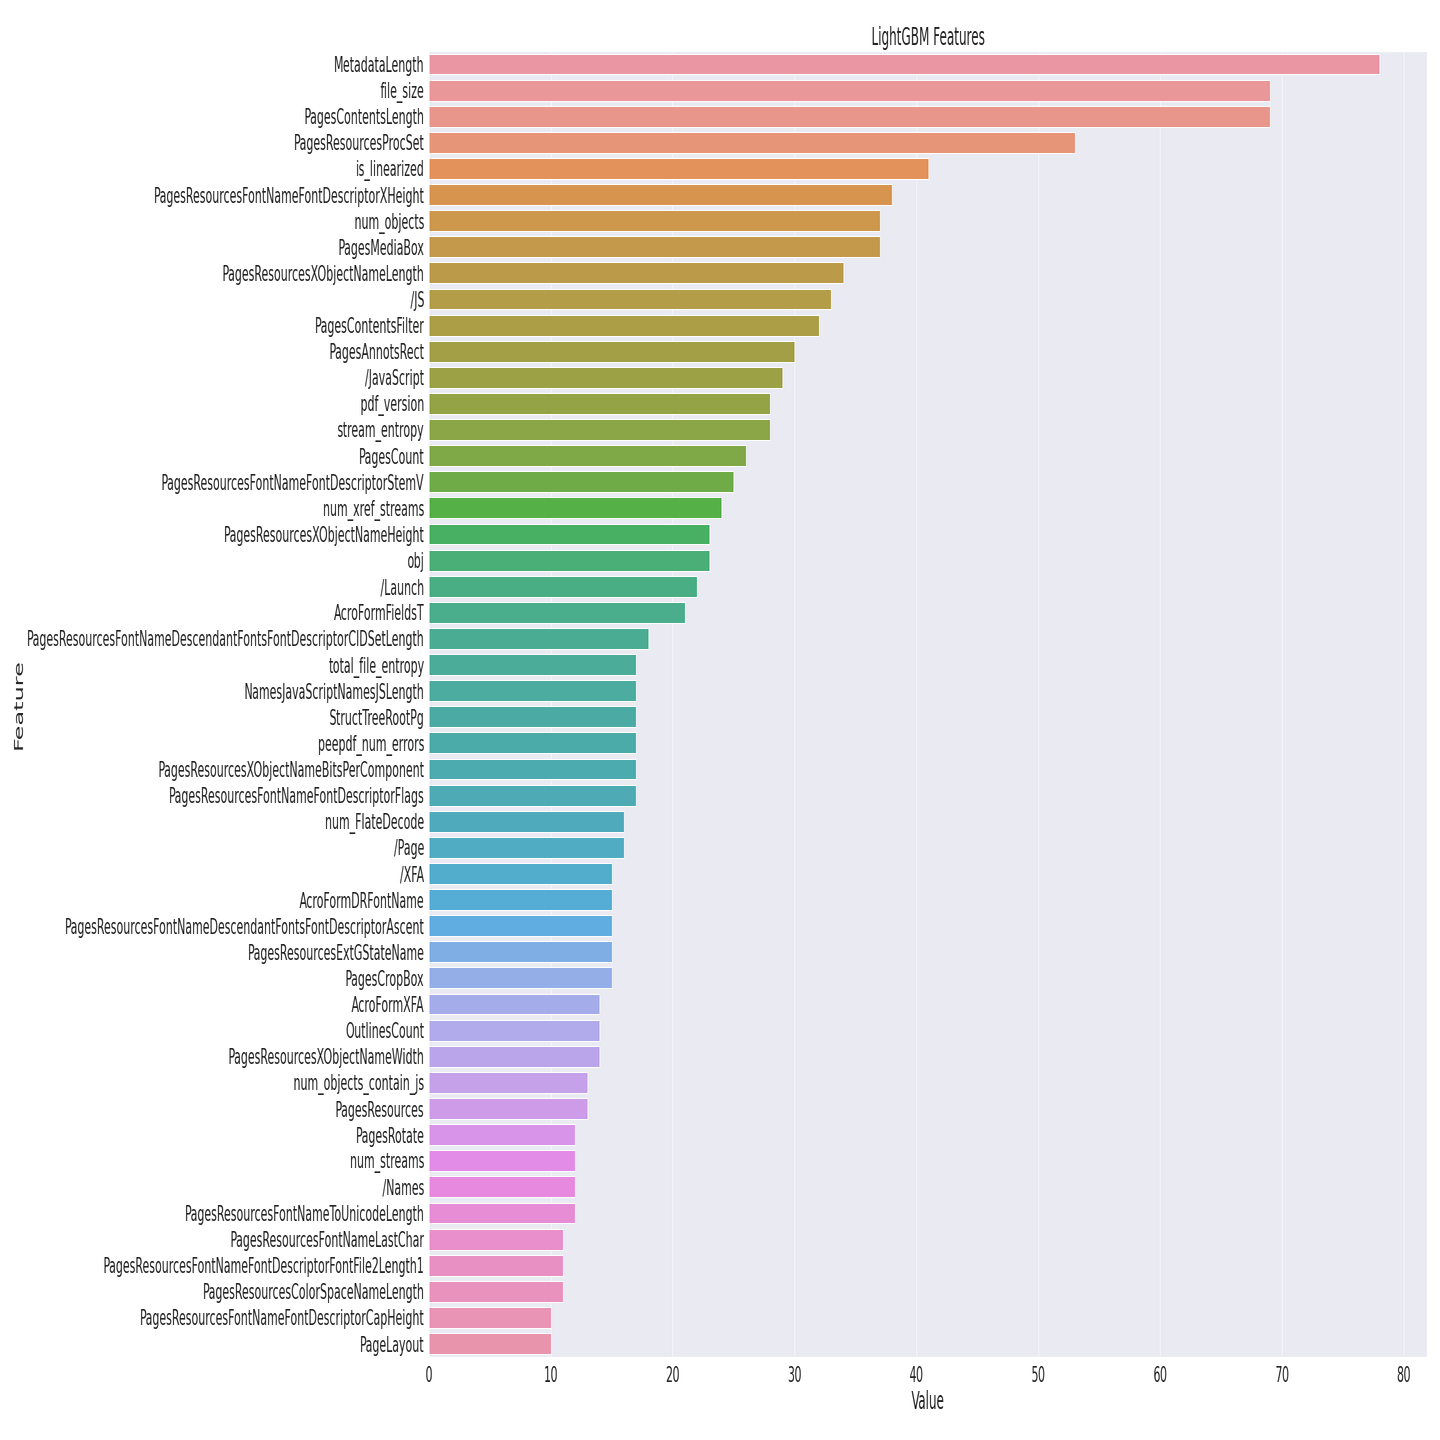
\includegraphics[width=\linewidth]{./images/lgbm_importances-01.png}
	\caption{Biểu đồ 50 đặc trưng có độ quan trọng cao nhất trong các đặc trưng thống kê và đường dẫn cấu trúc.}
	\label{fig:lgbm_importances-01}
\end{figure}

Quan sát kết quả xếp hạng độ quan trọng các đặc trưng, có thể thấy các đặc trưng liên quan đến kích thước dữ liệu, nội dung trong tệp PDF mang lại độ quan trọng cao nhất, ví dụ như Metadata\slash Length, Pages\slash Contents\slash Length hay file\_size.

Ngoài ra một số đặc trưng liên quan đến đoạn mã javascript hay liên quan đến biểu mẫu tương tác AcroForm trong tài liệu PDF cũng mang lại sự hữu ích trong mô hình phân loại khi xuất hiện nhiều trong top 50 này, ví dụ \slash JS, \slash Javascript, AcroFormDRFontName, AcroFormXFA, AcroFormFieldsT, NamesJavascriptNameJSLength.

\subsection{So sánh kết quả khi điều chỉnh tham số và số lượng đặc trưng}
Như đã giới thiệu, ở thí nghiệm này, tôi sử dụng optuna để tự động điều chỉnh tham số đầu vào cho thuật toán học máy LightGBM. Qua quá trình lặp lại với nhiều lần điều chỉnh, tôi đã chọn được bộ tham số mang lại kết quả tốt nhất cho thuật toán. Dưới đây là biểu đồ so sánh kết quả kiểm định trên các mô hình LightGBM tốt nhất được ghi lại tại lần thử thứ 10, 100 và 1000. [ref{fig}] Kết quả đã cho thấy hiệu quả của việc điều chỉnh tham số trong mô hình học máy.

\begin{figure}[H]
	\centering
	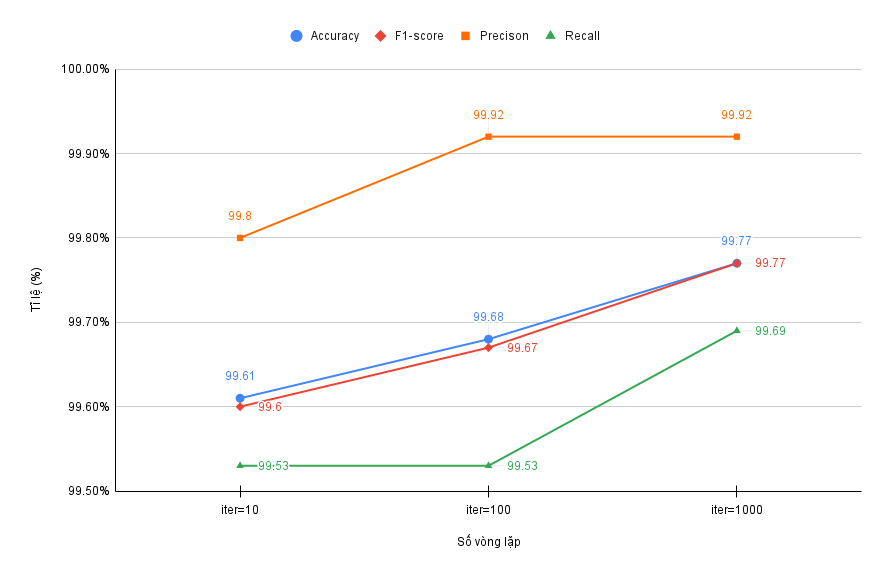
\includegraphics[width=\linewidth]{./images/exp1_trials.png}
	\caption{Biểu đồ so sánh kết quả điều chỉnh tham số thuật toán LightGBM qua các lần lặp trên tập kiểm chứng}
	\label{fig:exp1_trials}
\end{figure}

Bên cạnh việc điều chỉnh các tham số, tôi tiếp tục thử nghiệm thuật toán với việc điều chỉnh số lượng đặc trưng từ tập đặc trưng ban đầu:

\begin{itemize}
	\item
	      Hình []: chỉ sử dụng các đặc trưng thống kê, và thực hiện thay đổi số lượng đặc trưng, kết quả cho thấy việc sử dụng toàn bộ tập đặc trưng thống kê mang lại kết quả tốt nhất với độ chính xác 99.41\%
	\item
	      Hình []: chỉ sử dụng các đặc trưng đường dẫn cấu trúc, và thực hiện thay đổi số lượng đặc trưng, kết quả cho thấy việc sử dụng toàn bộ tập đặc trưng cấu trúc cây mang lại kết quả tốt nhất với độ chính xác 99.5\%
	\item
	      Hình []: thay đổi số lượng đặc trưng trên toàn bộ đặc trưng đã trích xuất được (bao gồm cả đặc trưng thống kê và đặc trưng cấu trúc cây). Kết quả cũng mang tại độ chính xác tốt nhất là 99.77\% khi sử dụng toàn bộ đặc trưng.
\end{itemize}

Việc sử dụng nhiều hơn các đặc trưng bằng thực nghiệm trên đã chứng minh là mang lại kết quả tốt hơn trên mô hình học máy LightGBM.

\begin{figure}[H]
	\centering
	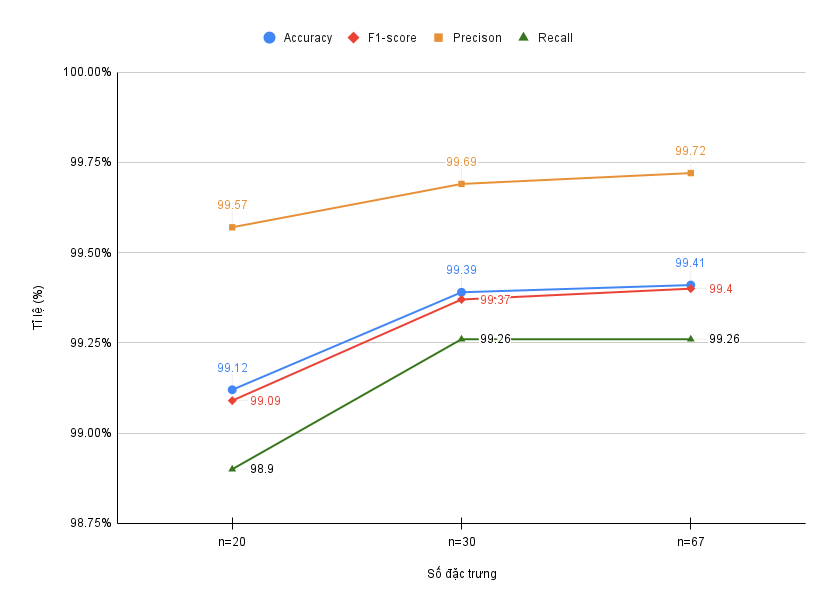
\includegraphics[width=\linewidth]{./images/exp1_top_all_general_feat.png}
	\caption{Biểu đồ so sánh mô hình khi sử dụng số lượng đặc trưng tăng dần từ tập đặc trưng thống kê.}
	\label{fig:exp1_top_all_general_feat}
\end{figure}

\begin{figure}[H]
	\centering
	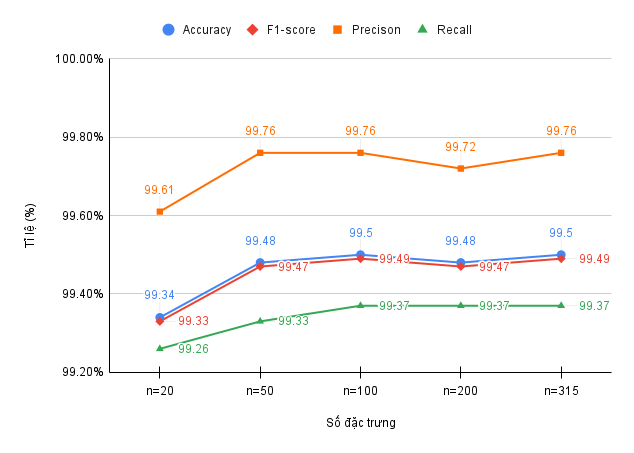
\includegraphics[width=\linewidth]{./images/exp1_top_all_structual_path.png}
	\caption{Biểu đồ so sánh kết quả của mô hình khi sử dụng số lượng đặc trưng tăng dần từ tập đặc trưng cấu trúc cây}
	\label{fig:exp1_top_all_structual_path}
\end{figure}

\begin{figure}[H]
	\centering
	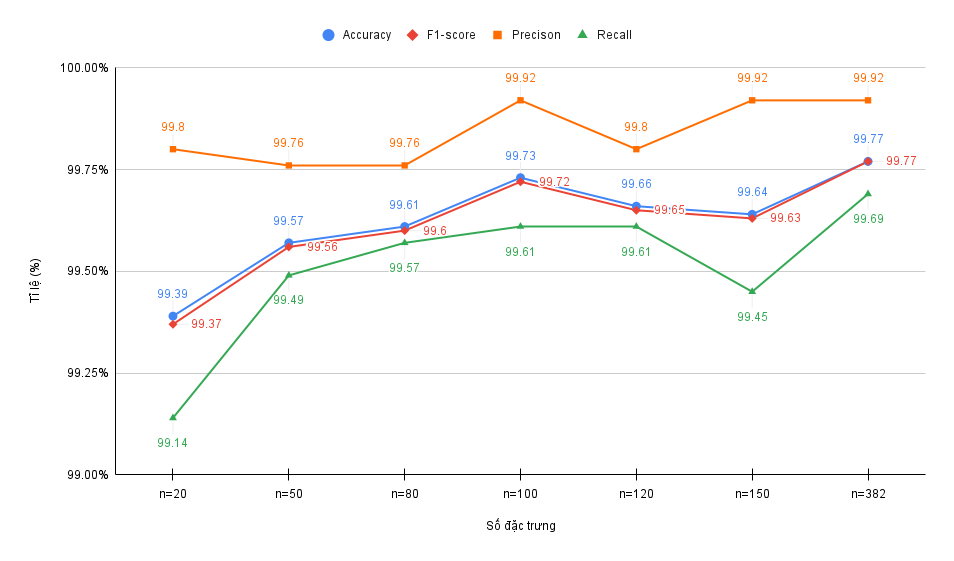
\includegraphics[width=\linewidth]{./images/exp1_top_all_feat.png}
	\caption{Biểu đồ so sánh kết quả của mô hình khi sử dụng số lượng đặc trưng tăng dần từ sự kết hợp các tập đặc trưng thống kê và đặc trưng cấu trúc cây.}
	\label{fig:exp1_top_all_feat}
\end{figure}

\subsection{So sánh kết quả khi kết hợp các loại đặc trưng}
Để đánh giá sự kết hợp của các đặc trưng thống kê và đường dẫn cấu trúc, thực hiện 3 thử nghiệm cho mô hình khi chỉ sử dụng tập đặc trưng thống kê, chỉ sử dụng tập đặc trưng cấu trúc cây và cuối cùng là sử dụng kết hợp hai loại đặc trưng này. Kết quả được biểu diễn trên biểu đồ dưới [], đã cho thấy một kết quả tốt nhất khi kết hợp các loại đặc trưng này với nhau.

Từ đó có thể kết luận, trong quy trình xác định một tài liệu PDF có độc hại hay không, việc phân tích và trích xuất nhiều loại đặc trưng nhất có thể, ở đây là các đặc trưng mang tính thống kê và các đặc trưng cấu trúc sẽ mang lại một mô hình phân loại đáng tin cậy hơn, thay vì chỉ sử dụng một số loại đặc trưng đơn lẻ.

\begin{figure}[H]
	\centering
	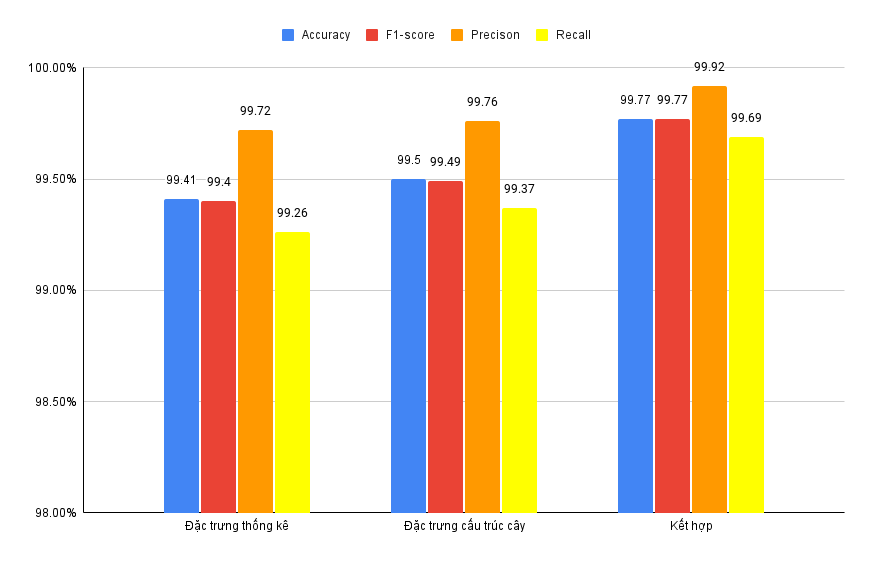
\includegraphics[width=\linewidth]{./images/exp1_compare_combination.png}
	\caption{Biểu đồ so sánh kết quả của mô hình khi sử dụng hai loại đặc trưng độc lập và khi kết hợp các đặc trưng thống kê và đặc trưng cấu trúc cây}
	\label{fig:exp1_compare_combination}
\end{figure}

\end{document}